%\input{preamble.txt}
%
%\begin{document}
\section{Introduction to Android}
\begin{itemize}
	\item Android
	\begin{itemize}
		\item Android is a platform comprising of three components
		\begin{itemize}
			\item An operating system
			\item A framework for developing applications
			\item Devices that run the Android operating system and the applications created
			for it
		\end{itemize}
		\item Android SDK
		\begin{itemize}
			\item A collection of libraries and tools that are needed for developing Android applications
		\end{itemize}
		\item Android Studio
		\begin{itemize}
			\item IDE for Android application development
		\end{itemize}
	\end{itemize}

	\item Android App Basics
	\begin{itemize}
		\item An Android app is a collection of screens, and each screen is comprised of a layout and an activity
		\begin{itemize}
			\item Layout: describes the appearance of a screen (written in XML)
			\item Activity: responsible for managing user interaction with the screen (written in java)
		\end{itemize}
		\item Folder structure:
		\begin{itemize}
			\begin{minipage}[t]{\widthof{Manifest file} + 1cm}
				\item Manifest file
				\item Java file
			\end{minipage}
			\begin{minipage}[t]{\widthof{Gradle scripts} + 1cm}
				\item Resource files
				\item Gradle scripts
			\end{minipage}
		\end{itemize}
	\end{itemize}
	\item The Manifest file
	\begin{itemize}
		\item It defines the structure and metadata of an application, its components, and its requirements
		\item Stored in the root of its project hierarchy as an XML file
	\end{itemize}

	\item Resources and resource IDs
	\begin{itemize}
		\item Resources are maintained in sub-directories of the \Verb|app/res| directory
		\begin{itemize}
			\item \Verb|res/layout|
			\item \Verb|res/values|
			\item Etc.
		\end{itemize}
		\item A resource can be accessed in the code using its resource ID (e.g. \Verb|R.layout.activity_main|)
		\begin{itemize}
			\item Android uses \Verb|R.java| to keep track of the resources used within the app
		\end{itemize}
	\end{itemize}

	\item View
	\begin{itemize}
		\item Most GUI components are instances of the \textbf{View} class or one of its subclasses
		\begin{itemize}
			\item e.g. Button, EditText, ImageView, etc.
		\end{itemize}
		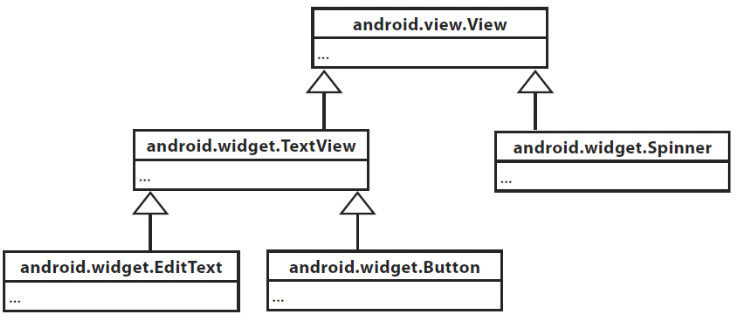
\includegraphics[scale=0.7]{View.png}
	\end{itemize}

	\newpage
	\item View Group
	\begin{itemize}
		\item A special type of view that can contain other views
		\item A layout is a type of view group\\
		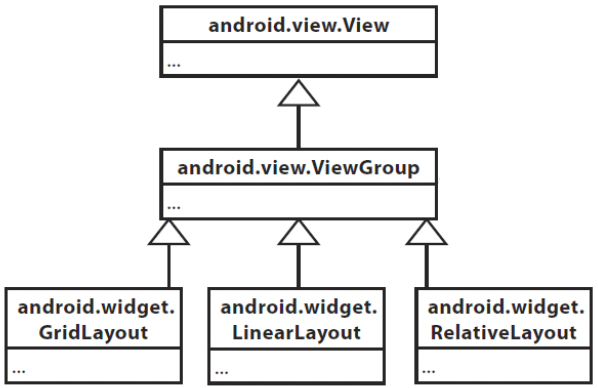
\includegraphics[scale=0.7]{ViewGroup.png}
	\end{itemize}

	\item Common GUI compnents
	\begin{itemize}
		\begin{minipage}[t]{\widthof{TextView} + 1cm}
			\item TextView
			\item EditText
			\item Button
		\end{minipage}
		\begin{minipage}[t]{\widthof{Spinner} + 1cm}
			\item Switch
			\item Spinner
			\item Toast
		\end{minipage}
	\end{itemize}

	\item Intents
	\begin{itemize}
		\item An intent is an object that can be used to bind activities together at runtime
		\begin{itemize}
			\item If one activity wants to start a second activity, it does it by sending an intent to Android. Android will start the second activity and pass it the intent
		\end{itemize}
		\item Data can be passed between activities using intent extras
		\begin{itemize}
			\item e.g. \Verb|intent.putExtra("message", value);|
		\end{itemize}
	\end{itemize}
\end{itemize}

%\end{document}